\chapter{The Cosmic Microwave Backgound}

\section{The Expanding Universe and the \texorpdfstring{$\Lambda$}{LAMBDA-}CDM Model}
\subsection{The Hubble's Law}\label{ss:hubbleslaw}

In 1929, Edwin Hubble examined the relationship between the distances of
some galaxies and their radial velocities, inferred from their \emph{redshifts},
and formulated an empirical law, which states direct proportionality
between these two quantities (\autoref{fig:hubbleslaw}):

\begin{equation}\label{eq:hubble_law}
        \vb{v} = H_0 \vb{d}
\end{equation}

where $H_0$ is the \emph{Hubble constant}.

\begin{figure}
        \centering
        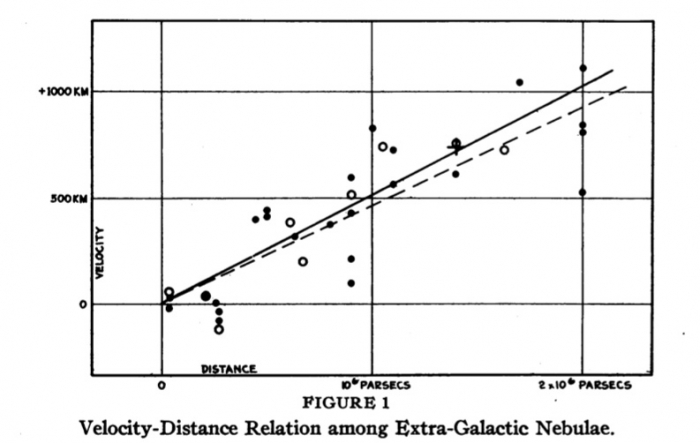
\includegraphics[width=\textwidth]{hubbleslaw}
        \caption{Hubbles Law}
        \label{fig:hubbleslaw}
\end{figure}

The observed \emph{redshifts} couldn't be explained by the proper motion of
the galaxies, instead this phenomenon was caused by the continuos expansion
of our universe.

An expanding universe was first theorized by Friedmann in 1922, before Hubble's
observations, as a consequence of the field equations of the theory of the
\emph{General Relativity} (GR). The starting point of Friedmann derivation was
an elegant and powerful assumption about the structure of our universe:
the \emph{Cosmological Principle}.

\subsection{The Cosmological Principle}\label{ss:cosmological_principle}

The matter in the universe we observe is clustered in gravitationally bound
structures, but observations at large scale (\SI{> 100}{\mega\parsec}) shows
that the place we call home appears to obey the \emph{Cosmological
Principle}:  

\begin{principle}[Cosmological Principle]
        On the largest scales, the universe is spatially homogeneous and isotropic.
\end{principle}

Note that this principle is valid for every possible observer in the
universe. We see an homogeneous and isotropic universe from our planet, and
we believe that any other observer in the universe does: there's no special
place in our universe.

There are two main piece of evidence for the cosmological principle:

\begin{itemize}
        \item The \emph{Comsmic Microwave Background Radiation} (CMB): an almost
        uniform sea of photons which fills all space and provides a snapshot of the
        universe at \num{\sim 380000} years after its birth. The CMB
        presents small fluctuations in temperature with a characteristic
        scale:

        \begin{equation}
                \frac{\var{T}}{T} \sim \num{e-5}
        \end{equation}

        \item A relevant number of \emph{redshift surveys} show that the
        distribution of stars looks increasengly smooth on larger scales.
\end{itemize}

The acceptance of such a profound statement it's the prologue to the
description of the geometry of \emph{spacetime}. 

\section{The CMB Radiation}

\begin{figure}
        \centering
        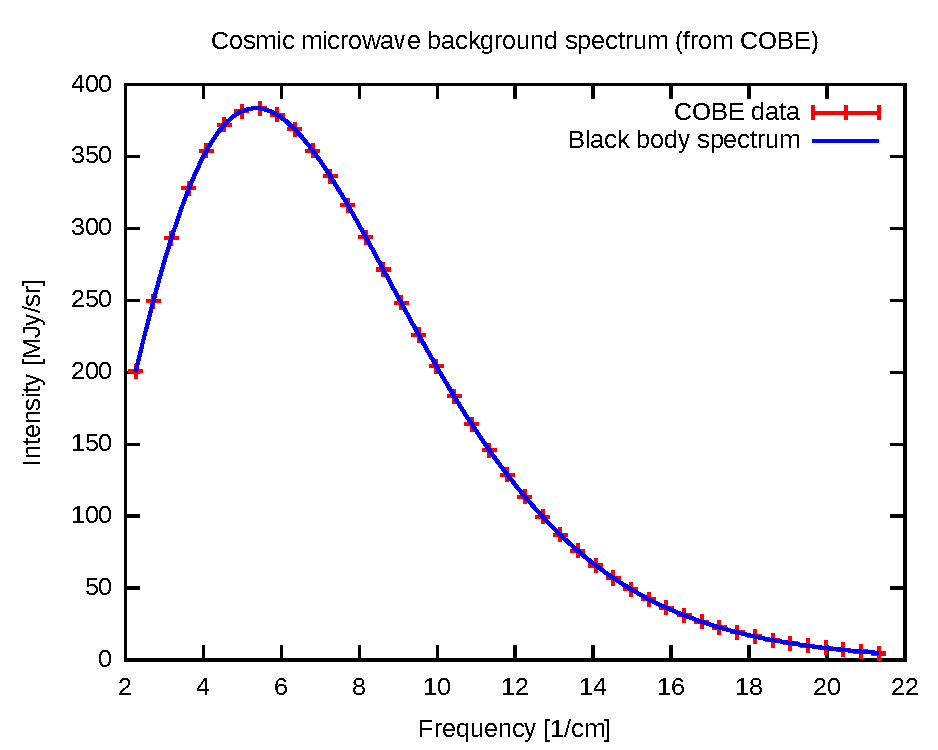
\includegraphics[width=\textwidth]{CMB_Spectrum_COBE}
        \caption{CMB Spectrum COBE}
        \label{fig:cmb_spectrum_cobe}
\end{figure}

\section{The CMB Temperature Anisotropies}

\begin{figure}
        \centering
        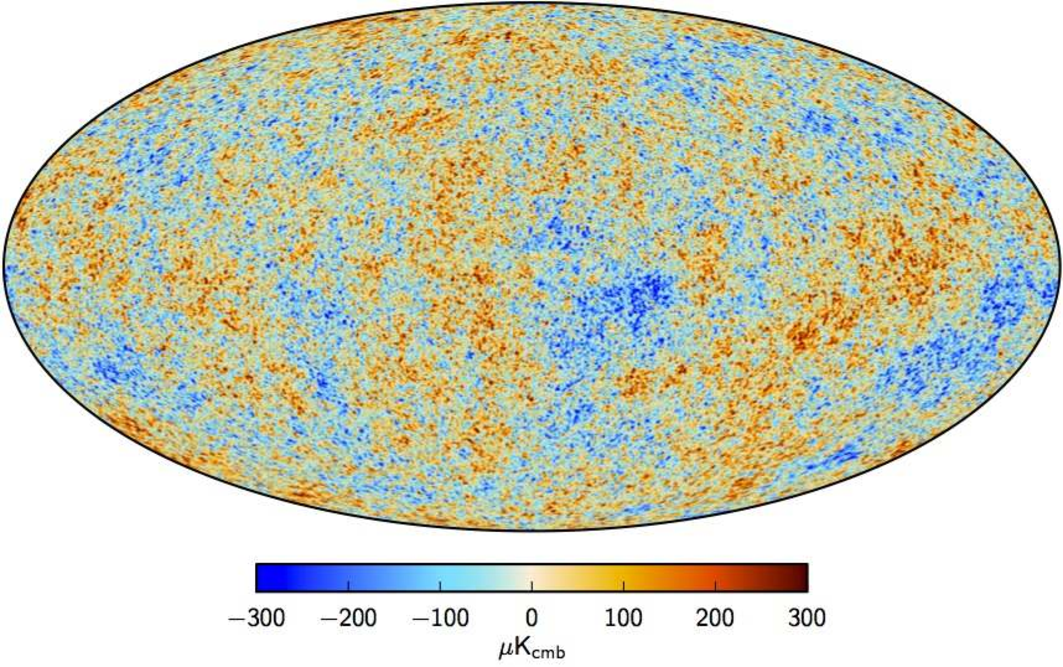
\includegraphics[width=\textwidth]{Planck_CMB}
        \caption{CMB Anisotropies Planck}
        \label{fig:plack_cmb}
\end{figure}

\section{The CMB Polarization}
